\documentclass[11pt,a4paper]{article}
\usepackage[margin=1in]{geometry}
\usepackage[T1]{fontenc}
\usepackage[utf8]{inputenc}
\usepackage{lmodern}
\usepackage{hyperref}
\usepackage{enumitem}
\usepackage{array}
\usepackage{longtable}
\usepackage{booktabs}
\usepackage{xurl}
\usepackage{tikz}
\usepackage{float}
\usetikzlibrary{arrows.meta, positioning, shapes.geometric}

\hypersetup{colorlinks=true,linkcolor=blue,urlcolor=blue}
\newcommand{\codepath}[1]{\path{#1}}
\setlength{\tabcolsep}{4pt}
\renewcommand{\arraystretch}{1.15}
\tikzset{
  box/.style={rectangle, draw, rounded corners, align=center, inner sep=3pt, minimum width=36mm},
  decision/.style={diamond, draw, aspect=2.2, align=center, inner sep=2pt},
  line/.style={-Latex}
}

\title{Document 2: Reference Datasets --- Phase-1}
\author{SIT Engine Architecture}
\date{\today}

\begin{document}
\maketitle
\tableofcontents
\newpage

\section{Purpose \& Scope}
\subsection*{Role of Pinned Datasets in Anchoring Correctness}
Pinned datasets are the deterministic input contract for semantic regression testing. They ensure that engine changes are evaluated against stable trace/mask fixtures rather than moving inputs.

\subsection*{Relation to Engine Version and Output Schema}
Phase-1 manifest now links dataset bundle and engine contract explicitly:
\begin{itemize}[leftmargin=*]
  \item \texttt{dataset\_version}
  \item \texttt{engine.name}
  \item \texttt{engine.version}
  \item \texttt{engine.schema\_version}
\end{itemize}
This linkage binds replay expectations to a specific SIT engine + schema surface.

Phase-0 baseline provenance: the original reference implementation ran on the Tenstorrent Wormhole testbench; parity traces can be normalized for Phase-1 replay through \codepath{Phase-1/phase0_trace_to_sit.py}.
\begin{itemize}[leftmargin=*]
  \item Source repo: \url{git@github.com:Srinidhi-Magesh08/Tenstorrent_test_raw_files.git}
  \item Baseline branch/commit: \texttt{main} @ \texttt{4512ce4e1a689f64c866160bf1f8e7e5e3e2ec89}
  \item Baseline run artifact: \codepath{phase0_golden/tt_run_2026-02-09/raw_profiler/profile_log_device.csv}
  \item Run header baseline: \texttt{ARCH=wormhole\_b0}, \texttt{CHIP\_FREQ[MHz]=1000}, \texttt{Max Compute Cores=64}
\end{itemize}

\section{Dataset Structure \& Contents}
\subsection*{What Each Dataset Contains}
Current Phase-1 bundle contains:
\begin{itemize}[leftmargin=*]
  \item traces: \codepath{Phase-1/datasets/traces/*.csv}
  \item includes direct Phase-0 Wormhole-derived sample: \codepath{datasets/traces/trace_F_phase0_wormhole_sample.csv}
  \item residency masks: \codepath{Phase-1/datasets/residency/*.csv}
  \item control manifest: \codepath{Phase-1/datasets/manifest.json}
\end{itemize}

Trace rows are normalized interval-like state events consumed by the baseline adapter/engine path. Residency files encode \([start\_us, end\_us)\) masks per core.

\subsection*{Versioning and Storage Layout (parquet/json context)}
Current pinned dataset storage is \textbf{CSV + JSON manifest}:
\begin{itemize}[leftmargin=*]
  \item JSON: manifest metadata and replay config
  \item CSV: trace/mask payload
\end{itemize}

Parquet currently applies to \textbf{exported outputs} (\texttt{windows\_v1.parquet}) via Phase-1 export, not to pinned dataset source bundle.

\subsection*{Immutability Guarantees and Enforcement}
Present guarantees:
\begin{itemize}[leftmargin=*]
  \item inputs are version-tagged in manifest,
  \item committed in git,
  \item validated through deterministic golden replay in CI.
\end{itemize}

Current enforcement model is procedural (version bump + CI replay), not cryptographic (no file checksum/signature fields in manifest yet).

\section{How Datasets Are Used}
\subsection*{Which Tests and Invariants Consume Datasets}
\begin{itemize}[leftmargin=*]
  \item \codepath{Phase-1/tests/run_golden_suite.py}: consumes traces + masks from manifest and executes all replay modes.
  \item \codepath{Phase-1/tests/check_invariants.py}: enforces semantic invariants over each replay output.
\end{itemize}

\subsection*{How Datasets Link to Specific Engine Version}
Manifest \texttt{engine} block links bundle expectations to engine/schema contract. Golden suite always runs \texttt{sit\_engine\_phase1.py}; together with manifest linkage this creates version-aware replay traceability.

\subsection*{Cross-Checks and Python Tests Already Executed}
Dataset-consumption checks executed in current environment:
\begin{longtable}{@{}>{\raggedright\arraybackslash}p{0.50\textwidth} >{\raggedright\arraybackslash}p{0.10\textwidth} >{\raggedright\arraybackslash}p{0.34\textwidth}@{}}
\toprule
\textbf{Executed Command} & \textbf{Result} & \textbf{Dataset Linkage Evidence} \\
\midrule
\endhead
\texttt{python3.9 tests/run\_golden\_suite.py --outdir /tmp/phase1\_golden\_py39} & PASS & Manifest traces + masks consumed;\\35 summary artifacts generated \\
\texttt{python3 tests/run\_golden\_suite.py --outdir golden\_out} & PASS & Same manifest-driven replay path\\validated with default interpreter \\
\texttt{python3.9 cli.py export --in /tmp/phase1\_export\_check --schema v1} & PASS & Output schema materialization\\validated for dataset-derived run \\
\bottomrule
\end{longtable}

Observed replay aggregation from pinned dataset bundle:
\begin{itemize}[leftmargin=*]
  \item traces in manifest: 8
  \item modes per trace: 5 (\texttt{base}, \texttt{all}, \texttt{skip\_w0}, \texttt{partial}, \texttt{exact\_boundary})
  \item total summary artifacts: 40
\end{itemize}

This demonstrates that pinned datasets are actively consumed by validation, not merely stored as static files.

\subsection*{Process for Adding/Updating a Dataset}
\begin{enumerate}[leftmargin=*]
  \item Add new trace/mask files under \texttt{datasets/traces} or \texttt{datasets/residency}.
  \item Update \texttt{datasets/manifest.json} (\texttt{traces}, masks, and version fields).
  \item Bump \texttt{dataset\_version}; adjust \texttt{engine} linkage if engine/schema expectation changed.
  \item Run golden suite locally.
  \item Merge only after CI pass.
\end{enumerate}

\section{Implementation Detail}
\subsection*{Directory Structure}
Current implemented structure is:
\begin{itemize}[leftmargin=*]
  \item \codepath{Phase-1/datasets/manifest.json}
  \item \codepath{Phase-1/datasets/traces/}
  \item \codepath{Phase-1/datasets/residency/}
\end{itemize}

Note: directories like \texttt{datasets/reference} or \texttt{datasets/pinned} are not currently used; manifest-driven structure above is the authoritative implementation.

\subsection*{Manifest Fields}
\begin{longtable}{>{\raggedright\arraybackslash}p{0.28\textwidth} >{\raggedright\arraybackslash}p{0.66\textwidth}}
\toprule
\textbf{Field} & \textbf{Meaning} \\
\midrule
\endhead
\texttt{dataset\_version} & Version tag for pinned dataset bundle. \\
\texttt{engine.name} & Engine identifier (Phase-1 SIT engine). \\
\texttt{engine.version} & Engine version linked to this dataset expectation. \\
\texttt{engine.schema\_version} & Output schema version linkage. \\
\texttt{phase0\_baseline} & Provenance block for Tenstorrent Wormhole baseline repo/commit/run metadata. \\
\texttt{window\_us\_default} & Default replay window size used by golden suite. \\
\texttt{traces[]} & Trace files included in replay set. \\
\texttt{residency\_masks\{\}} & Named mask files used by mode-specific validation passes. \\
\bottomrule
\end{longtable}

\subsection*{How CLI Pipeline Loads and Validates Datasets at Runtime}
\begin{itemize}[leftmargin=*]
  \item CLI ingest/classify/export pipeline (\codepath{Phase-1/cli.py}) operates on user-specified inputs and generated run manifests.
  \item Golden dataset replay is executed by \codepath{tests/run_golden_suite.py}, which loads \codepath{datasets/manifest.json}.
  \item Runtime output contract validation is enforced during export via \codepath{schema/v1.py} validators in \texttt{cmd\_export}.
\end{itemize}

\section{Flowchart}
\begin{figure}[H]
  \centering
  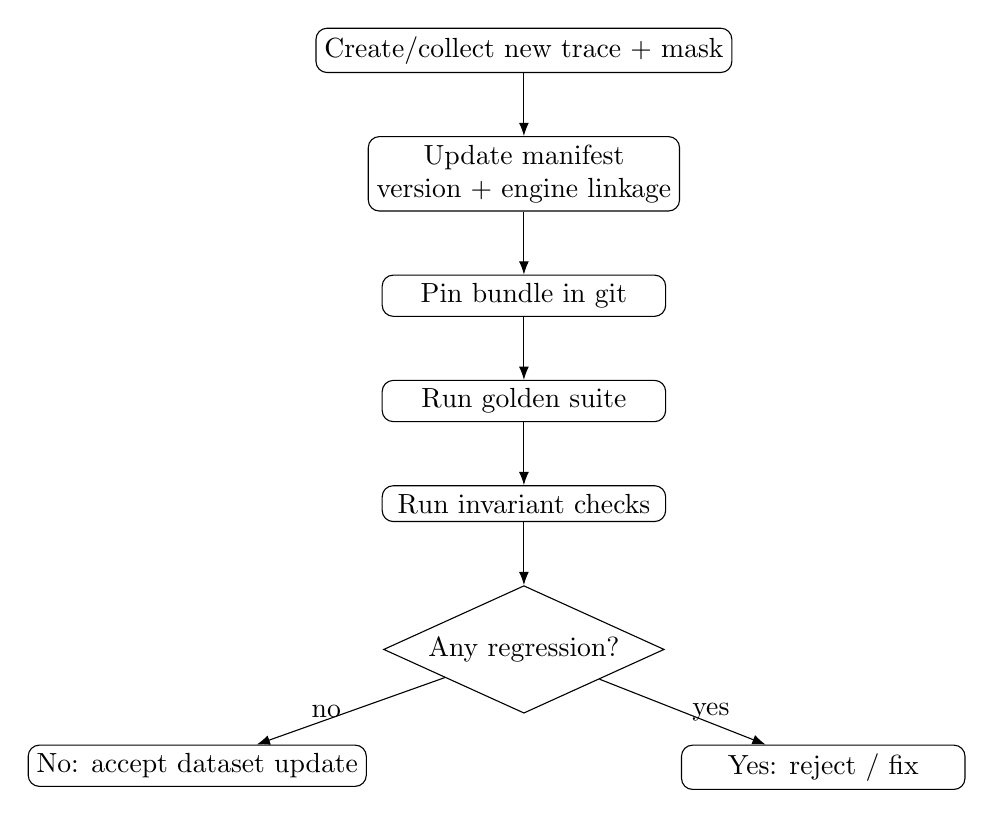
\begin{tikzpicture}[node distance=8mm and 11mm]
    \node[box] (c) {Create/collect new trace + mask};
    \node[box, below=of c] (v) {Update manifest\\version + engine linkage};
    \node[box, below=of v] (p) {Pin bundle in git};
    \node[box, below=of p] (g) {Run golden suite};
    \node[box, below=of g] (i) {Run invariant checks};
    \node[decision, below=of i] (d) {Any regression?};
    \node[box, below left=of d] (ok) {No: accept dataset update};
    \node[box, below right=of d] (fail) {Yes: reject / fix};
    \draw[line] (c) -- (v);
    \draw[line] (v) -- (p);
    \draw[line] (p) -- (g);
    \draw[line] (g) -- (i);
    \draw[line] (i) -- (d);
    \draw[line] (d) -- node[left]{no} (ok);
    \draw[line] (d) -- node[right]{yes} (fail);
  \end{tikzpicture}
  \caption{Reference Dataset Lifecycle and Regression Gate}
\end{figure}

\section{Done-When Criteria Mapping}
Done-when target: \textbf{Dataset linked to engine version.}

\begin{longtable}{@{}>{\raggedright\arraybackslash}p{0.34\textwidth} >{\raggedright\arraybackslash}p{0.32\textwidth} >{\raggedright\arraybackslash}p{0.20\textwidth}@{}}
\toprule
\textbf{Requirement} & \textbf{Repository Evidence} & \textbf{Status} \\
\midrule
\endhead
Versioned dataset bundle exists & \codepath{dataset_version} in \codepath{datasets/manifest.json} & Met \\
Dataset explicitly linked to engine version & \codepath{engine.name/version/schema_version} in manifest & Met \\
Bundle consumed by automated replay & \begin{tabular}[t]{@{}l@{}}\codepath{tests/run_golden_suite.py}\\loads manifest\end{tabular} & Met \\
Bundle validated semantically & \begin{tabular}[t]{@{}l@{}}\codepath{tests/check_invariants.py}\\per replay output\end{tabular} & Met \\
CI gate uses bundle-driven replay & \codepath{.github/workflows/phase1-ci.yml} & Met \\
\bottomrule
\end{longtable}

\end{document}
